\documentclass[a4paper,11pt]{article}
\usepackage{amsmath,amsthm,amsfonts,amssymb,amscd,amstext,vmargin,graphics,graphicx,tabularx,multicol} \usepackage[french]{babel}
\usepackage[utf8]{inputenc}  
\usepackage[T1]{fontenc} 
\usepackage[T1]{fontenc}
\usepackage{amsmath,amssymb}
\usepackage{pstricks-add,tikz,tkz-tab,variations}
\usepackage[autolanguage,np]{numprint} 
\usepackage{color}
\usepackage{ulem}

\setmarginsrb{1.5cm}{0.5cm}{1cm}{0.5cm}{0cm}{0cm}{0cm}{0cm} %Gauche, haut, droite, haut
\newcounter{numexo}
\newcommand{\exo}[1]{\stepcounter{numexo}\noindent{\bf Exercice~\thenumexo} : \marginpar{\hfill /#1}}
\reversemarginpar


\newcounter{enumtabi}
\newcounter{enumtaba}
\newcommand{\q}{\stepcounter{enumtabi} \theenumtabi)  }
\newcommand{\qa}{\stepcounter{enumtaba} (\alph{enumtaba}) }
\newcommand{\initq}{\setcounter{enumtabi}{0}}
\newcommand{\initqa}{\setcounter{enumtaba}{0}}

\newcommand{\be}{\begin{enumerate}}
\newcommand{\ee}{\end{enumerate}}
\newcommand{\bi}{\begin{itemize}}
\newcommand{\ei}{\end{itemize}}
\newcommand{\bp}{\begin{pspicture*}}
\newcommand{\ep}{\end{pspicture*}}
\newcommand{\bt}{\begin{tabular}}
\newcommand{\et}{\end{tabular}}
\renewcommand{\tabularxcolumn}[1]{>{\centering}m{#1}} %(colonne m{} centrée, au lieu de p par défault) 
\newcommand{\tnl}{\tabularnewline}

\newcommand{\trait}{\noindent \rule{\linewidth}{0.2mm}}
\newcommand{\hs}[1]{\hspace{#1}}
\newcommand{\vs}[1]{\vspace{#1}}

\newcommand{\N}{\mathbb{N}}
\newcommand{\Z}{\mathbb{Z}}
\newcommand{\R}{\mathbb{R}}
\newcommand{\C}{\mathbb{C}}
\newcommand{\Dcal}{\mathcal{D}}
\newcommand{\Ccal}{\mathcal{C}}
\newcommand{\mc}{\mathcal}

\newcommand{\vect}[1]{\overrightarrow{#1}}
\newcommand{\ds}{\displaystyle}
\newcommand{\eq}{\quad \Leftrightarrow \quad}
\newcommand{\vecti}{\vec{\imath}}
\newcommand{\vectj}{\vec{\jmath}}
\newcommand{\Oij}{(O;\vec{\imath}, \vec{\jmath})}
\newcommand{\OIJ}{(O;I,J)}

\newcommand{\bmul}[1]{\begin{multicols}{#1}}
\newcommand{\emul}{\end{multicols}}


\newcommand{\reponse}[1][1]{%
\multido{}{#1}{\makebox[\linewidth]{\rule[0pt]{0pt}{20pt}\dotfill}
}}

\newcommand{\titre}[5] 
% #1: titre #2: haut gauche #3: bas gauche #4: haut droite #5: bas droite
{
\noindent #2 \hfill #4 \\
#3 \hfill #5

\vspace{-1.6cm}

\begin{center}\rule{6cm}{0.5mm}\end{center}
\vspace{0.2cm}
\begin{center}{\large{\textbf{#1}}}\end{center}
\begin{center}\rule{6cm}{0.5mm}\end{center}
}



\begin{document}
\pagestyle{empty}
\titre{Contrôle 1 : Proportionnalité, transformations, relatifs et fractions }{Nom}{Prénom}{Date}{Classe}

\begin{flushleft}
\begin{tabular}{|m{9.5cm}|m{1.25cm}|m{1.25cm}|m{1.25cm}|m{1.25cm}|m{1.25cm}|}
\hline 
\textbf{Compétences} & \begin{center}
\textbf{N.E.}
\end{center} & \begin{center}
\textbf{M.I.}
\end{center} & \begin{center}
\textbf{M.F.}
\end{center}  & \begin{center}
\textbf{M.S.}
\end{center} & \begin{center}
\textbf{T.B.M.}
\end{center} \\ 
\hline 
Extraire d'un document les informations utiles, les reformuler, les organiser, les confronter à ses connaissances &  &  & & &\\
\hline 
Décomposer un problème en sous-problèmes &  &  & & &\\
\hline



\end{tabular} 
\end{flushleft}

\textit{N.E = Non évalué ; M.I. = Maîtrise insuffisante ; M.F. = Maîtrise fragile ; M.S. = Maîtrise satisfaisante ; T.B.M. = Très bonne maîtrise}\\

\vspace*{0.3cm}

\exo{3} \textit{(Proportionnalité)}


Un avionneur donne la consommation moyenne de l'un de ses avions moyen courrier grâce au graphique ci-dessous.

\begin{center}


\includegraphics[scale=0.7]{avionneur.eps} 
\end{center}

\qa La quantité de kérosène et le temps passé dans les airs  sont-ils proportionnels  ? Expliquer.\\

\qa A l'aide du graphique, donner le plus précisément possible le temps que l'avion passe dans les airs avec 30 t de kérosène.\\


\qa	A l'aide du graphique, donner le plus précisément possible la quantité de kérosène nécessaire pour faire voler un avion pendant 2 heures 30.\\





\vspace*{0.5cm}

\exo{7} \textit{(Les fractions)}

Calculer les expressions suivantes en détaillant toutes vos étapes de calculs et \textbf{simplifier les résultats si possible} :

















\bmul{3}
$L=10+(-17,1)-(-8)-9,9+22$\\

$E = \dfrac{5}{4} - \dfrac{10}{12}$\\ 


\columnbreak



$R = \dfrac{4}{5} - \dfrac{19}{5} + \dfrac{11}{5}$\\

$F = \dfrac{23}{4} - \left( \dfrac{1}{2} - \dfrac{1}{4}   \right)$\\ 


\columnbreak

$T=2-\dfrac{20}{7}$

$M = \left(  \dfrac{7}{6}+\dfrac{2}{3} \right)- \left(\dfrac{11}{9} + \dfrac{7}{18}\right)$\\ 


\emul

\vspace*{0.5cm}


\exo{3} \textit{(Les fractions)}

Dans une carafe d'un litre, on mélange $\dfrac{1}{2}$ L de jus d'orange, $\dfrac{1}{20}$ L de jus de citron, $\dfrac{1}{10}$ L de jus de pamplemousse et $\dfrac{2}{5}$ L de sucre de canne.\\

Quelle quantité de boisson obtient-on ? La carafe va-t-elle déborder ? Pourquoi ? (\textbf{Justifier votre réponse par des calculs.)}\\

\newpage

\vspace*{0.5cm}


\exo{4} \textit{(Les transformations)}\\

\bmul{2}
\initq
\q On considère l'hexagone ABCDEF de centre O représenté ci-contre.\\

\qa Quelle est l'image du quadrilatère CDEO par la symétrie de centre O?\\

\qa Quelle est l'image du segment [AO] par la symétrie d'axe (CF)?\\

\qa On considère la rotation de centre O qui transforme le triangle OAB en le triangle OCD.\\
Quelle est l'image du triangle BOC par cette rotation ?\\


\columnbreak

\includegraphics[scale=0.8]{hexagone1.eps} 

\emul
\vspace*{0.25cm}


\bmul{2}
\q La figure ci-contre représente un pavage dont le motif
de base a la même forme que l'hexagone ci-dessus. On
a numéroté certains de ces hexagones.\\

$\rightarrow$ \textbf{Quelle est l'image de l'hexagone 14 par la translation qui transforme l'hexagone 2 en l'hexagone
12 ?}\\

\columnbreak

\includegraphics[scale=0.75]{nidabeille.eps} 


\emul


\vspace*{0.5cm}
\exo{3} \textbf{Sur le sujet,} \\

\initqa
\noindent \qa construire l'image du nombre 2 000 par la rotation de  centre  O,  d'angle  90\degre,  dans  le sens inverse des aiguilles d'une montre;\\

\noindent \qa construire l'image du nombre 2 000 par la translation qui transforme le point A en C.\\

\vspace*{0.5cm}

\includegraphics[scale=1=0.8]{exobrevet.eps} \\
\vspace*{1.5cm}

\end{document}
